\section{Verwendete KI-Software}
\label{anhang:ki}
Im Rahmen der Erstellung dieser Arbeit wurden KI-basierte Werkzeuge ausschließlich unterstützend eingesetzt.
Tabelle~\ref{tab:ki} dokumentiert die verwendeten Tools, ihren Einsatzbereich und den Bearbeitungsumfang gemäß den Hinweisen von Prof.\ Diersen.
Alle KI-generierten Inhalte wurden inhaltlich überprüft, gegen wissenschaftliche Primärquellen abgeglichen und in eigenen Worten in den Text integriert.
Eine unmittelbare Übernahme generierter Passagen erfolgte nicht.
\begin{table}[htbp]
\centering
\caption{Übersicht verwendeter KI-Software}
\label{tab:ki}
\begin{tabularx}{\textwidth}{p{3.8cm}XX}
\toprule
\textbf{Tool} & \textbf{Einsatzbereich} & \textbf{Umfang} \\
\midrule
Claude Code (Anthropic),\newline VS-Code-Extension
  & Python-Code-Unterstützung (Omniverse-Extension), Strukturierung und Verwaltung des Literatur- und Dokumentenordners
  & kontinuierlich, alle Inhalte inhaltlich geprüft und überarbeitet \\
GWDG Chat AI
  & Strukturierung Inhaltsverzeichnis, sprachliche Glättung
  & punktuell, gegengeprüft \\
LanguageTool\newline (LanguageTool GmbH)
  & KI-gestützte Grammatik- und Stilprüfung auf Deutsch, Erkennung stilistischer Mängel im Fließtext
  & punktuell, rein korrekturlesend \\
Duden Mentor\newline (Bibliographisches Institut)
  & Orthografische und grammatikalische Kontrolle deutschsprachiger Texte auf Regelwerks-Basis
  & punktuell, rein orthografisch \\
Ragnar (app.ragnar.build),\newline AI Text- \& Image-to-CAD
  & Erzeugung eines CAD-Modells der Schutzverkleidung für den \enquote{Mr.\,Fusion}-Reaktor am DeLorean-Modell im Pick-and-Place-Szenario des Dobot Magician anhand des Prompts \enquote{Erstelle einen Hohlzylinder mit einem Innendurchmesser von 13\,mm, einem Außendurchmesser von 14\,mm und einer Höhe von 10\,mm. Eine Seite ist geschlossen. Die Kanten an der offenen Seite sind abgerundet.}
  & einmalig genutzt, Ergebnis entsprach direkt den Anforderungen, keine Nachbearbeitung notwendig \\
Zoo Text-to-CAD\newline (Zoo Studio)
  & Erzeugung eines CAD-Modells des Sauggreifers für den Dobot Magician anhand des Prompts \enquote{Erstelle ein CAD-Modell des abgebildeten Sauggreifers} mit einem Screenshot aus der Dobot-Anleitung als Bildvorlage
  & einmalig genutzt, Ergebnis inhaltlich geprüft \\
\bottomrule
\end{tabularx}
\end{table}

\section{Reproduktions-Anleitung (Auszug)}
\label{anhang:repro}
Der vollständige Reproduktions-Leitfaden ist als digitales Übergabepaket im LFP-Repository hinterlegt. Tabelle~\ref{tab:repro} fasst die sieben Schritte mit den jeweils erzeugten Artefakten zusammen.
\begin{table}[htbp]
\centering
\caption{Sieben-Schritte-Modell zur Reproduktion eines Digitalen Zwillings}
\label{tab:repro}
\begin{tabularx}{\textwidth}{clX}
\toprule
\textbf{Nr.} & \textbf{Schritt} & \textbf{Artefakt} \\
\midrule
1 & Anforderungs- und Schnittstellenanalyse        & Anforderungsliste, Schnittstellenmatrix \\
2 & CAD-Aufbereitung und USD-Export                & \texttt{.usd}-Stage \\
3 & Definition kinematischer Strukturen            & Articulation-Konfiguration \\
4 & Auswahl Middleware                             & Architekturdiagramm \\
5 & Implementierung der Datenkopplung              & Python-Extension, Konfigurationsdateien \\
6 & Validierung                                    & Messprotokolle, Latenzwerte \\
7 & Übergabe und Versionierung                     & Git-Repository, Dokumentation \\
\bottomrule
\end{tabularx}
\end{table}

\section{Auszug aus der URDF-Beschreibung des Dobot}
\label{anhang:urdf}
\begin{lstlisting}[basicstyle=\ttfamily\footnotesize,frame=single,breaklines=true,caption={Auszug aus der URDF-Datei \texttt{dobot\_magician.urdf}}]
<robot name="dobot_magician">
  <link name="base_link">
    <visual>
      <geometry>
        <mesh filename="meshes/base.stl"/>
      </geometry>
    </visual>
    <inertial>
      <mass value="1.2"/>
      <inertia ixx="0.01" ixy="0" ixz="0"
               iyy="0.01" iyz="0" izz="0.01"/>
    </inertial>
  </link>
  <joint name="joint1" type="revolute">
    <parent link="base_link"/>
    <child  link="link1"/>
    <axis xyz="0 0 1"/>
    <limit lower="-2.62" upper="2.62"
           effort="10" velocity="3.14"/>
  </joint>
  <!-- weitere Glieder und Gelenke ... -->
</robot>
\end{lstlisting}

\section{Küster Omniverse Tutorial -- Reproduktionsanleitung}
\label{anhang:omniverse_tutorial}
Die nachfolgende Anleitung dokumentiert vollständig den Prozess der Erstellung eines Digitalen Zwillings mit NVIDIA Omniverse und NVIDIA Isaac Sim, wie er im Rahmen dieser Arbeit erarbeitet wurde. Sie richtet sich an Studierende und Mitarbeitende des LFP, die den Prozess eigenständig nachvollziehen möchten.

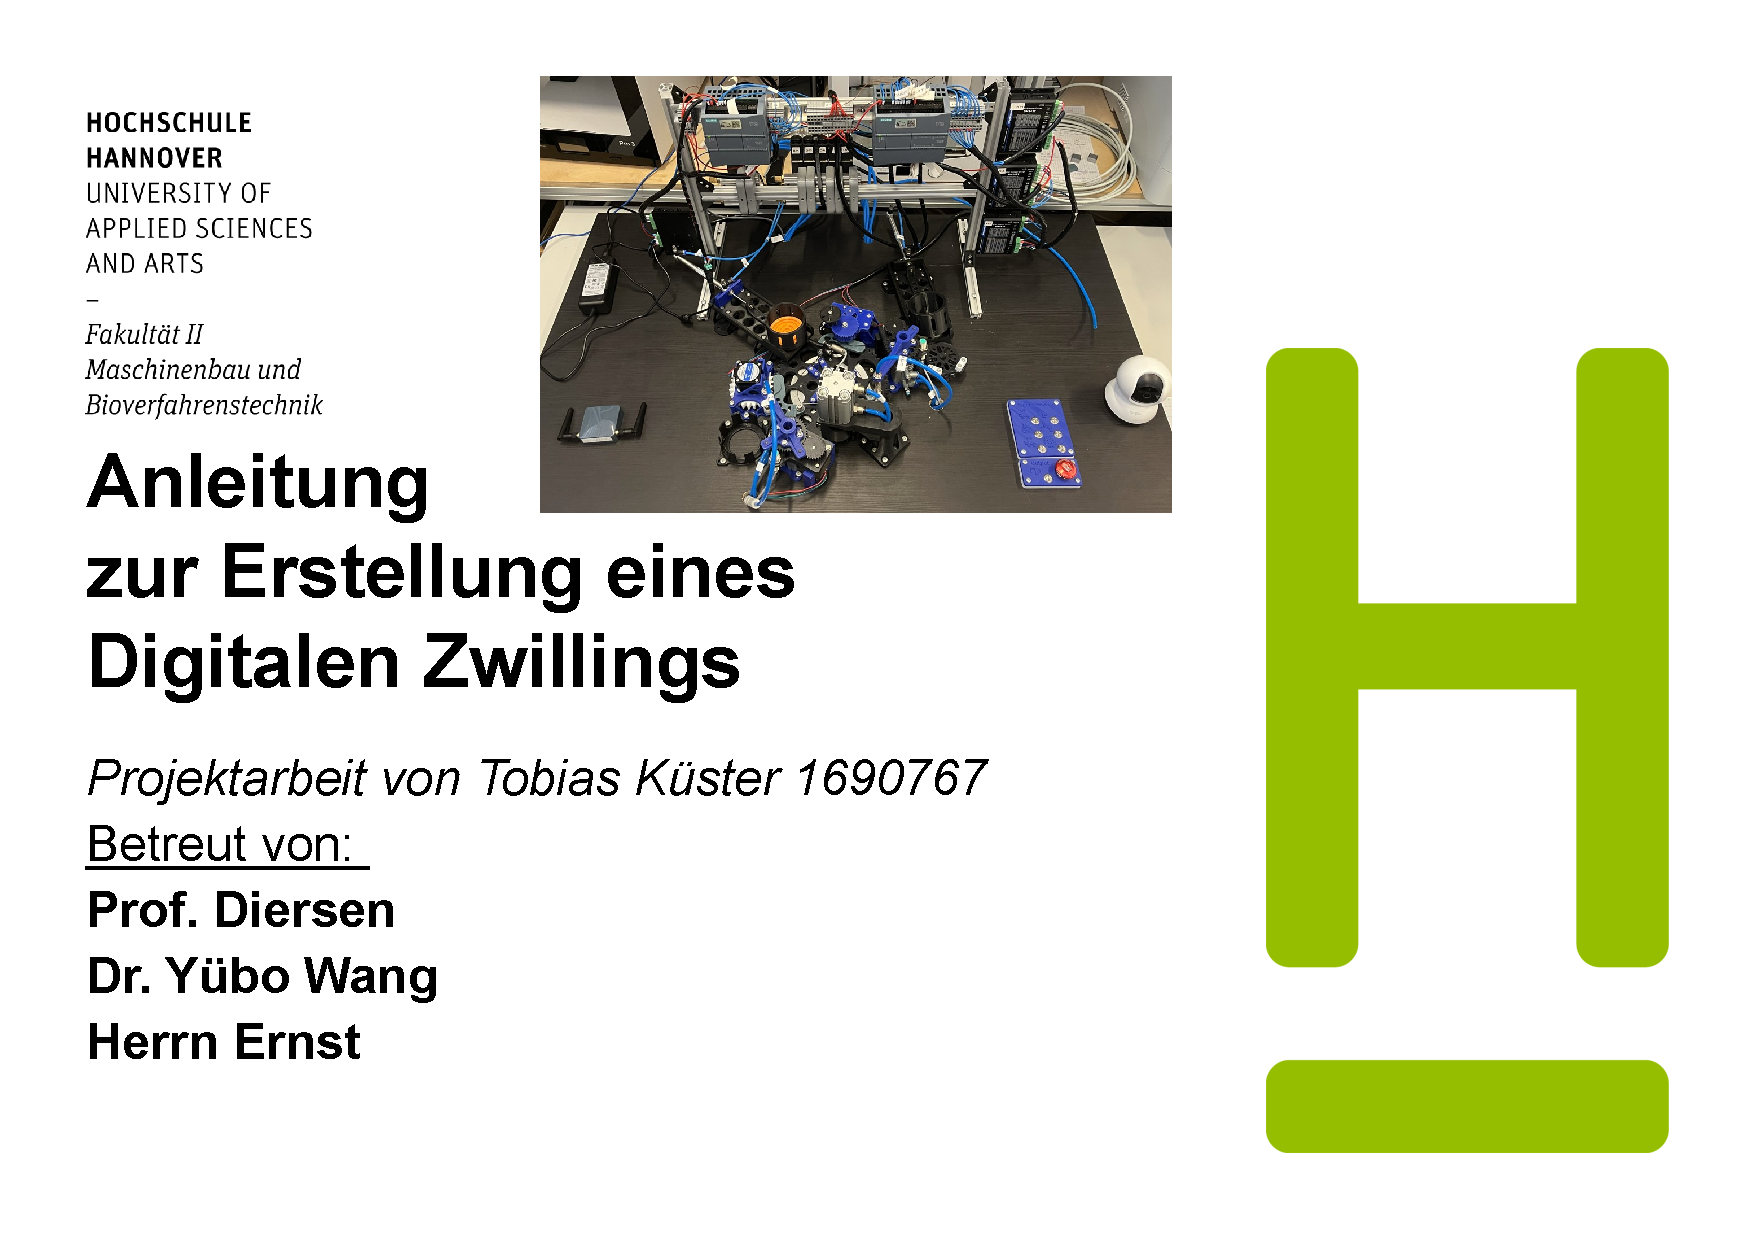
\includepdf[pages=-,pagecommand={\thispagestyle{plain}},fitpaper=true]{Doku_Hinweise_Leitfaeden/Kuester_Omniverse_Tutorial.pdf}

\section{Schnittstellenmatrix Maze Runner (Auszug)}
\label{anhang:schnittstellen}
\begin{table}[htbp]
\centering
\caption{Auszug aus der OPC-UA-Schnittstellenmatrix des Maze Runner}
\begin{tabularx}{\textwidth}{lllX}
\toprule
\textbf{Variable} & \textbf{Datentyp} & \textbf{Richtung} & \textbf{Beschreibung} \\
\midrule
\texttt{TableAngle}     & Float  & R   & Aktueller Drehwinkel des Rundtakttisches in Grad \\
\texttt{TableSpeed}     & Float  & R/W & Soll-/Ist-Drehzahl in U/min \\
\texttt{GripperState}   & Bool   & R/W & Pneumatischer Greifer geöffnet/geschlossen \\
\texttt{SensorStation1} & Bool   & R   & Induktiver Näherungsschalter Station 1 \\
\texttt{EmergencyStop}  & Bool   & R   & Status Not-Halt-Kreis \\
\bottomrule
\end{tabularx}
\end{table}
